\begin{appendices}

  \chapter{Hasil Uji Coba Kebenaran pada Situs SPOJ}
  \setcounter{figure}{0}
  \renewcommand{\thetable}{A.\arabic{table}}
  \renewcommand{\thefigure}{A.\arabic{figure}}
  
  \begin{figure}[H]
  	\centerline{ 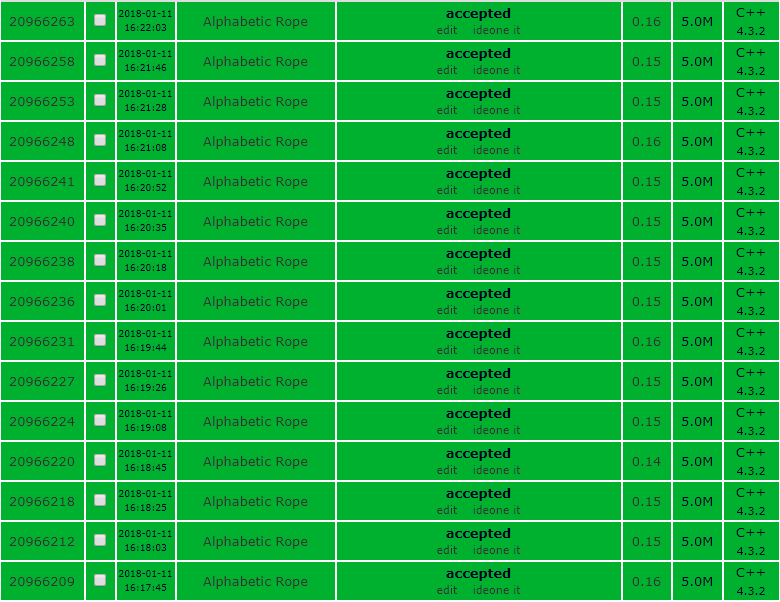
\includegraphics[scale=0.5]{assets/images/submission.png}}
  	\caption{Hasil Pengujian Sebanyak 15 Kali pada Situs Penilaian Daring SPOJ}
  	\label{figure:submission}
  \end{figure}
  
  \chapter{Hasil Uji Performa Penyelesaian Operasi 1 Menggunakan Struktur Data Rope dan Algorithma String}
  \setcounter{figure}{0}
  \renewcommand{\thetable}{B.\arabic{table}}
  \renewcommand{\thefigure}{B.\arabic{figure}}
  
  \begin{table} [H]
  \centering
	  \begin{tabular}{|c|c|c|c|}
		  \hline
		  \multirow{2}{*}{Panjang String} & Rope & Rope - pembanding & String\\
		  		  & Waktu (detik) & Waktu (detik) & Waktu (detik)\\ \hline
		  5000 & 0.04584	& 0.37512	& 0.21461\\ \hline
		  10000 & 0.04568	& 0.42488	& 0.27259\\ \hline
		  15000 & 0.04298	& 0.45005	& 0.32707\\ \hline
		  20000 & 0.04261	& 0.46458	& 0.40244\\ \hline
		  25000 & 0.04352	& 0.47984	& 0.46670\\ \hline
		  30000 & 0.04239	& 0.48971	& 0.53264\\ \hline
		  35000 & 0.04229	& 0.49920	& 0.60791\\ \hline
		  40000 & 0.04324	& 0.50714	& 0.68570\\ \hline
		  45000 & 0.04716	& 0.51634	& 0.77109\\ \hline
		  50000 & 0.04239	& 0.52379	& 0.87648\\ \hline
		  55000 & 0.04225	& 0.53031	& 0.98290\\ \hline
		  60000 & 0.04218	& 0.53815	& 1.11034\\ \hline
		  65000 & 0.04262	& 0.54562	& 1.24909\\ \hline
		  70000 & 0.04251	& 0.55366	& 1.26256\\ \hline
		  75000 & 0.04286	& 0.56215	& 1.24042\\ \hline
		  80000 & 0.04524	& 0.57252	& 1.31375\\ \hline
		  85000 & 0.04271	& 0.58538	& 1.40470\\ \hline
		  90000 & 0.04243	& 0.58756	& 1.49502\\ \hline
		  95000 & 0.04246	& 0.60007	& 1.59853\\ \hline
		  100000 & 0.04229	& 0.60352	& 1.69388\\ \hline
	  \end{tabular}\caption{Tabel Hasil Uji Coba pada Operasi 1 dengan Jumlah \textit{Query} tetap dan Panjang \textit{String} Bertambah}
	  \label{tab:operasi1string}
  \end{table}
  
  \begin{table} [H]
    \centering
  	  \begin{tabular}{|c|c|c|c|}
  		  \hline
  		  \multirow{2}{*}{Banyak Query} & Rope & Rope - pembanding & String\\
  		    		  & Waktu (detik) & Waktu (detik) & Waktu (detik)\\ \hline
  		  5000	& 0.00212	& 0.02678	& 0.09447\\ \hline
  		  10000	& 0.00426	& 0.05573	& 0.17078\\ \hline
  		  15000	& 0.00634	& 0.08553	& 0.25521\\ \hline
  		  20000	& 0.00851	& 0.11321	& 0.33912\\ \hline
  		  25000	& 0.01048	& 0.14259	& 0.42499\\ \hline
  		  30000	& 0.01272	& 0.17272	& 0.50647\\ \hline
  		  35000	& 0.01482	& 0.20204	& 0.59519\\ \hline
  		  40000	& 0.01777	& 0.23304	& 0.67729\\ \hline
  		  45000	& 0.01924	& 0.27471	& 0.75871\\ \hline
  		  50000	& 0.02168	& 0.29658	& 0.84541\\ \hline
  		  55000	& 0.02483	& 0.32535	& 0.92717\\ \hline
  		  60000	& 0.02616	& 0.3547	& 1.01493\\ \hline
  		  65000	& 0.02785	& 0.38604	& 1.09944\\ \hline
  		  70000	& 0.02959	& 0.41976	& 1.18202\\ \hline
  		  75000	& 0.03220	& 0.44713	& 1.26605\\ \hline
  		  80000	& 0.03432	& 0.47656	& 1.35644\\ \hline
  		  85000	& 0.03614	& 0.50967	& 1.43311\\ \hline
  		  90000	& 0.03923	& 0.53864	& 1.51598\\ \hline
  		  95000	& 0.04044	& 0.56934	& 1.60935\\ \hline
  		  100000	& 0.04229	& 0.60352	& 1.69388\\ \hline
  	  \end{tabular}\caption{Tabel Hasil Uji Coba pada Operasi 1 dengan Panjang \textit{String} tetap dan Jumlah \textit{Query} Bertambah}
  	  \label{tab:operasi1query}
    \end{table}
    
  \chapter{Hasil Uji Performa Penyelesaian Operasi 2 Menggunakan Struktur Data Rope dan String}
  \setcounter{figure}{0}
  \renewcommand{\thetable}{C.\arabic{table}}
  \renewcommand{\thefigure}{C.\arabic{figure}}
  
  \begin{table}[h]
  \centering
	  \begin{tabular}{|c|c|c|c|}
		  \hline
		  \multirow{2}{*}{Panjang String} & Rope & Rope - pembanding & String\\
		  		  & Waktu (detik) & Waktu (detik) & Waktu (detik)\\ \hline
		  5000	& 0.08046	& 0.45924	& 0.15061\\ \hline
		  10000	& 0.07907	& 0.51843	& 0.21968\\ \hline
		  15000	& 0.07804	& 0.54997	& 0.30699\\ \hline
		  20000	& 0.07941	& 0.56391	& 0.42457\\ \hline
		  25000	& 0.07919	& 0.58758	& 0.52275\\ \hline
		  30000	& 0.08137	& 0.59856	& 0.64959\\ \hline
		  35000	& 0.07963	& 0.6151	& 0.80127\\ \hline
		  40000	& 0.0807	& 0.6351	& 0.96337\\ \hline
		  45000	& 0.07853	& 0.64935	& 1.12678\\ \hline
		  50000	& 0.07917	& 0.66312	& 1.33048\\ \hline
		  55000	& 0.08274	& 0.67976	& 1.5374\\ \hline
		  60000	& 0.07855	& 0.68753	& 1.74437\\ \hline
		  65000	& 0.07848	& 0.70459	& 1.9582\\ \hline
		  70000	& 0.08031	& 0.71008	& 1.93652\\ \hline
		  75000	& 0.07816	& 0.73011	& 2.12236\\ \hline
		  80000	& 0.07947	& 0.73807	& 2.27391\\ \hline
		  85000	& 0.08009	& 0.7404	& 2.4679\\ \hline
		  90000	& 0.07838	& 0.74922	& 2.63696\\ \hline
		  95000	& 0.07819	& 0.76165	& 2.7606\\ \hline
		  100000	& 0.08379	& 0.76779	& 2.94229\\ \hline
	  \end{tabular}\caption{Tabel Hasil Uji Coba pada Operasi 2 dengan Jumlah \textit{Query} tetap dan Panjang \textit{String} Bertambah}
	  \label{tab:operasi2string}
  \end{table}
  
  \begin{table}[h]
    \centering
  	  \begin{tabular}{|c|c|c|c|}
 		  \hline
 		  \multirow{2}{*}{Banyak Query} & Rope & Rope - pembanding & String\\
 		    		  & Waktu (detik) & Waktu (detik) & Waktu (detik)\\ \hline
  		  5000	& 0.0021	& 0.03094	& 0.15582\\ \hline
  		  10000	& 0.00422	& 0.06923	& 0.31249\\ \hline
  		  15000	& 0.0082	& 0.10347	& 0.45776\\ \hline
  		  20000	& 0.01235	& 0.14144	& 0.60343\\ \hline
  		  25000	& 0.01652	& 0.17569	& 0.75053\\ \hline
  		  30000	& 0.02187	& 0.21542	& 0.89214\\ \hline
  		  35000	& 0.02437	& 0.25814	& 1.06315\\ \hline
  		  40000	& 0.02868	& 0.29264	& 1.19422\\ \hline
  		  45000	& 0.03337	& 0.32757	& 1.33897\\ \hline
  		  50000	& 0.03724	& 0.37407	& 1.48473\\ \hline
  		  55000	& 0.04161	& 0.41413	& 1.62678\\ \hline
  		  60000	& 0.04647	& 0.45708	& 1.77913\\ \hline
  		  65000	& 0.04975	& 0.48762	& 1.92705\\ \hline
  		  70000	& 0.05391	& 0.5315	& 2.06298\\ \hline
  		  75000	& 0.05869	& 0.57248	& 2.21603\\ \hline
  		  80000	& 0.06229	& 0.61257	& 2.35933\\ \hline
  		  85000	& 0.06674	& 0.65026	& 2.50408\\ \hline
  		  90000	& 0.07095	& 0.68927	& 2.64912\\ \hline
  		  95000	& 0.07366	& 0.74459	& 2.80072\\ \hline
  		  100000	& 0.08379	& 0.76779	& 2.94229\\ \hline
  	  \end{tabular}\caption{Tabel Hasil Uji Coba pada Operasi 2 dengan Panjang String tetap dan Jumlah Query Bertambah}
  	  \label{tab:operasi2query}
    \end{table}
    
  \chapter{Hasil Uji Performa Penyelesaian Operasi 3 Menggunakan Struktur Data Rope dan String}
  \setcounter{figure}{0}
  \renewcommand{\thetable}{D.\arabic{table}}
  \renewcommand{\thefigure}{D.\arabic{figure}}
  
  \begin{table}[h]
  \centering
	 \begin{tabular}{|c|c|c|c|}
		  \hline
		  \multirow{2}{*}{Panjang String} & Rope & Rope - pembanding & String\\
		  		  & Waktu (detik) & Waktu (detik) & Waktu (detik)\\ \hline
		  5000	& 0.05484	& 0.05753	& 0.06929\\ \hline
		  10000	& 0.05765	& 0.06085	& 0.06749\\ \hline
		  15000	& 0.05815	& 0.06444	& 0.06798\\ \hline
		  20000	& 0.06014	& 0.06593	& 0.06812\\ \hline
		  25000	& 0.06007	& 0.06808	& 0.06819\\ \hline
		  30000	& 0.06121	& 0.06983	& 0.06805\\ \hline
		  35000	& 0.06197	& 0.07425	& 0.07311\\ \hline
		  40000	& 0.06253	& 0.0781	& 0.06874\\ \hline
		  45000	& 0.06310	& 0.07199	& 0.06835\\ \hline
		  50000	& 0.06381	& 0.0733	& 0.06814\\ \hline
		  55000	& 0.06449	& 0.07532	& 0.06797\\ \hline
		  60000	& 0.06485	& 0.07707	& 0.0689\\ \hline
		  65000	& 0.06592	& 0.08287	& 0.07186\\ \hline
		  70000	& 0.06668	& 0.08182	& 0.07765\\ \hline
		  75000	& 0.06788	& 0.08158	& 0.06994\\ \hline
		  80000	& 0.07156	& 0.08723	& 0.06788\\ \hline
		  85000	& 0.07049	& 0.0875	& 0.06823\\ \hline
		  90000	& 0.07054	& 0.09047	& 0.06874\\ \hline
		  95000	& 0.07153	& 0.08684	& 0.06834\\ \hline
		  100000	& 0.07222	& 0.0871	& 0.07223\\ \hline
	  \end{tabular}\caption{Tabel Hasil Uji Coba pada Operasi 3 dengan Jumlah \textit{Query} tetap dan Panjang \textit{String} Bertambah}
	  \label{tab:operasi3string}
  \end{table}
  
  \begin{table}[h]
    \centering
  	  \begin{tabular}{|c|c|c|c|}
   		  \hline
   		  \multirow{2}{*}{Banyak Query} & Rope & Rope - pembanding & String\\
   		    		  & Waktu (detik) & Waktu (detik) & Waktu (detik)\\ \hline
  		  5000	& 0.00403	& 0.0046	& 0.00411\\ \hline
  		  10000	& 0.00753	& 0.00901	& 0.00729\\ \hline
  		  15000	& 0.01116	& 0.01278	& 0.01078\\ \hline
  		  20000	& 0.01524	& 0.01901	& 0.01501\\ \hline
  		  25000	& 0.01878	& 0.02309	& 0.01763\\ \hline
  		  30000	& 0.02204	& 0.02543	& 0.02134\\ \hline
  		  35000	& 0.02565	& 0.03114	& 0.02496\\ \hline
  		  40000	& 0.02920	& 0.03496	& 0.02786\\ \hline
  		  45000	& 0.03271	& 0.04112	& 0.03096\\ \hline
  		  50000	& 0.03638	& 0.04661	& 0.03399\\ \hline
  		  55000	& 0.04029	& 0.05072	& 0.03738\\ \hline
  		  60000	& 0.04361	& 0.05377	& 0.04412\\ \hline
  		  65000	& 0.04844	& 0.05963	& 0.04669\\ \hline
  		  70000	& 0.05078	& 0.06232	& 0.05085\\ \hline
  		  75000	& 0.05493	& 0.07118	& 0.05242\\ \hline
  		  80000	& 0.05782	& 0.06998	& 0.05502\\ \hline
  		  85000	& 0.06153	& 0.0758	& 0.05955\\ \hline
  		  90000	& 0.06514	& 0.08392	& 0.06156\\ \hline
  		  95000	& 0.06884	& 0.08232	& 0.06455\\ \hline
  		  100000	& 0.07222	& 0.0871	& 0.07223\\ \hline
  	  \end{tabular}\caption{Tabel Hasil Uji Coba pada Operasi 3 dengan Panjang String tetap dan Jumlah Query Bertambah}
  	  \label{tab:operasi3query}
    \end{table}

\end{appendices}